\chapter{Исследовательская часть}

В данном разделе приведены примеры работы алгоритма.

\section{Тестирование}

\begin{figure}[h]
	\centering
	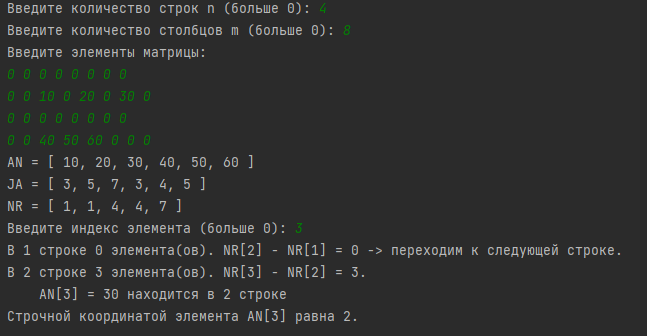
\includegraphics[width=0.85\textwidth]{img/test-01.png}
	\caption{Тест №1, поиск строчной координаты элемента под индексом 3, значение которого 30}
	\label{fig:test-01}
\end{figure}

\begin{figure}[h]
	\centering
	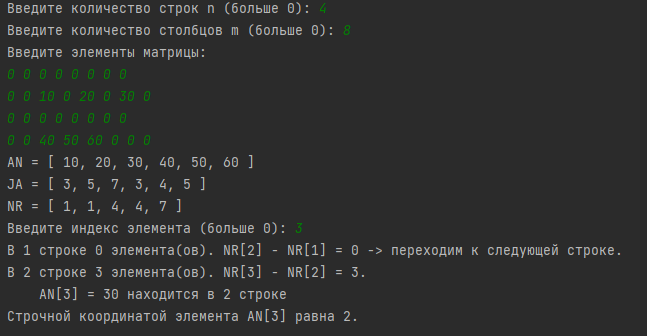
\includegraphics[width=0.85\textwidth]{img/test-01.png}
	\caption{Тест №2, поиск строчной координаты элемента под индексом 4, значение которого 40}
	\label{fig:test-02}
\end{figure}

\begin{figure}[h]
	\centering
	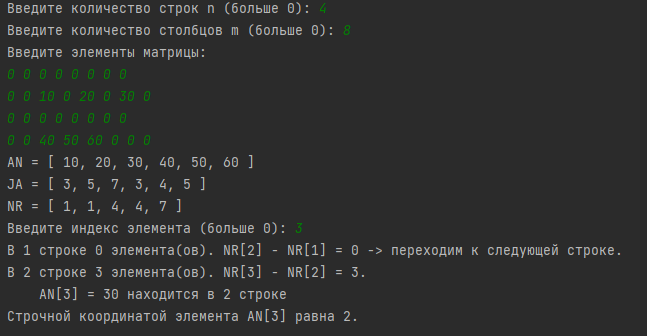
\includegraphics[width=0.85\textwidth]{img/test-01.png}
	\caption{Тест №3, поиск строчной координаты элемента c неверным индексом в массиве NR}
	\label{fig:test-03}
\end{figure}